\documentclass[handout]{beamer}

\usepackage{minted}
\usepackage[utf8]{inputenc}
\usepackage{graphicx}

\mode<presentation>{
  \usetheme{default}
}

\setbeamertemplate{navigation symbols}{}
\setbeamertemplate{footline}[frame number]

%% -------------------------------------------------------------------------- %%

\title{Declarative Internal DSLs in Lua}
\subtitle{A Game-Changing Experience}
\author{Alexander Gladysh, ag@logiceditor.com\\\textbf{L}ogic\textbf{E}ditor.com CTO, co-founder}
\date{Lua Workshop 2011}

%% -------------------------------------------------------------------------- %%

\begin{document}

\maketitle

%% -------------------------------------------------------------------------- %%

\begin{frame}

\frametitle{Outline}

\tableofcontents

\end{frame}

%% -------------------------------------------------------------------------- %%

\section{Introduction}

%% -------------------------------------------------------------------------- %%

\begin{frame}[fragile]

\frametitle{Internal Declarative DSL in Lua}

\begin{minted}{lua}
namespace:method "title"
{
  data = "here";
}
\end{minted}

\end{frame}

%% -------------------------------------------------------------------------- %%

\begin{frame}[fragile]

\frametitle{...Without sugar}

\begin{minted}{lua}
_G["namespace"]:method(
    "title"
  ) ({
    ["data"] = "here";
  })
\end{minted}

\end{frame}

%% -------------------------------------------------------------------------- %%

\begin{frame}[fragile]

\frametitle{Naïve implementation}

\begin{minted}{lua}
namespace = { }

namespace.method = function(self, name)
   return function(data)
    -- ...do something
    -- ...with name and data
  end
end
\end{minted}

\end{frame}

%% -------------------------------------------------------------------------- %%

\section{Ad-hoc approach}

%% -------------------------------------------------------------------------- %%

\begin{frame}[fragile]

\frametitle{Hypothetical UI description language}

\begin{minted}{lua}
ui:dialog "alert"
{
  ui:label "message";
  ui:button "OK"
  {
    on_click = function(self)
      self:close()
    end;
  };
}
\end{minted}

\end{frame}

%% -------------------------------------------------------------------------- %%

\begin{frame}[fragile]

\frametitle{UI description language "implementation", I}

\begin{minted}{lua}
function ui:label(title)
  return function(data)
    return GUI.Label:new(title, data)
  end
end

function ui:button(title)
  return function(data)
    return GUI.Button:new(title, data)
  end
end
\end{minted}

\end{frame}

%% -------------------------------------------------------------------------- %%

\begin{frame}[fragile]

\frametitle{UI description language "implementation", II}

\begin{minted}{lua}
function ui:dialog(title)
  return function(data)
    local dialog = GUI.Dialog:new(title)
    for i = 1, #data do
      dialog:add_child(data)
    end
    return dialog
  end
end
\end{minted}

\end{frame}

%% -------------------------------------------------------------------------- %%

\begin{frame}

\frametitle{Ad-hoc approach}

\begin{itemize}
\item[+] Easy to code simple stuff
\end{itemize}

But:

\begin{itemize}
\item[$-$] Easily grows out of control
\item[$-$] Difficult to reuse
\item[$-$] Hard to handle errors
\item[$-$] Hard to add new output targets
\end{itemize}

\end{frame}

%% -------------------------------------------------------------------------- %%

\section{A case study}

%% -------------------------------------------------------------------------- %%

\begin{frame}[fragile]

\frametitle{Practical example: HTTP handler}

\begin{minted}{lua}
api:url "/reverse"
{
  doc:description [[String reverser]]
  [[
    Takes a string and reverses it.
  ]];
  api:input { data:string "text" };
  api:output
  {
    data:node "result" { data:string "reversed" };
  };
  handler = function(param)
    return { reversed = param.text:reverse() }
  end;
}
\end{minted}

\end{frame}

%% -------------------------------------------------------------------------- %%

\begin{frame}

\frametitle{What do we want to get from that description?}

\begin{itemize}
\item \textbf{HTTP request handler itself}, with:
  \begin{itemize}
  \item Input validation
  \item Multi-format output serialization (JSON, XML, ...)
  \item Handler code static checks (globals, ...)
  \end{itemize}
\item \textbf{Documentation}
\item Low-level networking \textbf{client code}
\item Smoke \textbf{tests}
\end{itemize}

\end{frame}

%% -------------------------------------------------------------------------- %%

\begin{frame}[fragile]

\frametitle{Request handler: input validation}

\begin{minted}{lua}
local handler = function(checker, param)
  return
  {
    text = checker:string(param, "text");
  }
end

INPUT_LOADERS["/reverse.xml"] = handler
INPUT_LOADERS["/reverse.json"] = handler
\end{minted}

\end{frame}

%% -------------------------------------------------------------------------- %%

\begin{frame}[fragile]

\frametitle{Request handler: output serialization}

\begin{minted}{lua}
local build_formatter = function(fmt)
  return fmt:node("nil", "result")
  {
    fmt:attribute("reversed");
  }
end

OUTPUT["/reverse.xml"] = build_formatter(
    make_xml_formatter_builder()
  ):commit()

OUTPUT["/reverse.json"] = build_formatter(
    make_json_formatter_builder()
  ):commit()
\end{minted}

\end{frame}

%% -------------------------------------------------------------------------- %%

\begin{frame}[fragile]

\frametitle{Request handler: the handler itself}

\begin{minted}{lua}
-- Handler code is checked for access to illegal globals.
-- Legal globals are aliased to locals at the top.
-- Necessary require() calls are added automatically.

local handler = function(param)
  return
  {
    reversed = param.text:reverse();
  }
end

HANDLERS["/reverse.xml"] = handler;
HANDLERS["/reverse.json"] = handler;
\end{minted}

\end{frame}

%% -------------------------------------------------------------------------- %%

\begin{frame}[fragile]

\frametitle{Documentation}
\large{\textbf{/reverse.\{xml, json\}: String reverser}}

Takes a string and reverses it.

\textbf{IN}
\begin{semiverbatim}
  ?text=STRING
\end{semiverbatim}

\textbf{OUT}

\textit{XML:}

\begin{minted}{xml}
<result reversed="STRING" />
\end{minted}

\textit{JSON:}

\begin{minted}{javascript}
{ "result": { "reversed": "STRING" } }
\end{minted}

\end{frame}

%% -------------------------------------------------------------------------- %%

\begin{frame}[fragile]

\frametitle{Smoke tests}

\begin{minted}{lua}
test:case "/reverse.xml:smoke.ok" (function()
  local reply = assert(http.GET(
      TEST_HOST .. "/reverse.xml?text=Foo")
    ))
  assert(type(reply.result) == "table")
  assert(type(reply.result.reversed) == "string")
end)
\end{minted}

\end{frame}

%% -------------------------------------------------------------------------- %%

\begin{frame}

\frametitle{Too complicated for ad-hoc solution!}

\begin{center}
\resizebox{\paperheight * 9 / 10}{!}{
\includegraphics{spaghetticat.jpg}}
\end{center}

\end{frame}

%% -------------------------------------------------------------------------- %%

\section{The "proper" solution}

%% -------------------------------------------------------------------------- %%

\begin{frame}

\frametitle{The "proper" solution?}

\begin{itemize}
\item Should be easy to add a new target.
\item Should be reusable.
\item Should have nicer error reporting.
\end{itemize}

\end{frame}

%% -------------------------------------------------------------------------- %%

\begin{frame}

\frametitle{The process}

\begin{itemize}
\item Load data.
\item Validate correctness.
\item Generate output.
\end{itemize}

\end{frame}

%% -------------------------------------------------------------------------- %%

\begin{frame}[fragile]

\frametitle{Let's recap how our data looks like}

\begin{minted}{lua}
api:url "/reverse"
{
  doc:description [[String reverser]]
  [[
    Takes a string and reverses it.
  ]]
  api:input { data:string "text" };
  api:output
  {
    data:node "result" { data:string "reversed" };
  };
  handler = function(param)
    return { reversed = param.text:reverse() }
  end;
}
\end{minted}

\end{frame}

%% -------------------------------------------------------------------------- %%

\begin{frame}[fragile]

\frametitle{Surprise! It's a tree!}

\begin{minted}{lua}
{ id = "api:url", name = "/reverse";
  { id = "doc:description", name = "String reverser";
    text = "Takes a string and reverses it.";
  };
  { id = "api:input";
    { id = "data:string", name = "text" };
  };
  { id = "api:output";
    { id = "data:node", name = "result";
      { id = "data:string", name = "reversed" };
    };
    handler = function(param)
      return { reversed = param.text:reverse() }
    end;
  };
}
\end{minted}

\end{frame}

%% -------------------------------------------------------------------------- %%

\begin{frame}[fragile]

\frametitle{We need a loader that does this: (I)}

\begin{columns}

\begin{column}{0.5\textwidth}
\begin{minted}{lua}
namespace:method "title"
{
  data = "here";
}
\end{minted}
\end{column}

\begin{column}{0.05\textwidth}
$\Rightarrow$
\end{column}

\begin{column}{0.5\textwidth}
\begin{minted}{lua}
{
  id = "namespace:method";
  name = "title";
  data = "here";
}
\end{minted}
\end{column}

\end{columns}
\end{frame}

%% -------------------------------------------------------------------------- %%

\begin{frame}[fragile]

\frametitle{We need a loader that does this: (II)}

\begin{columns}

\begin{column}{0.5\textwidth}
\begin{minted}{lua}
namespace:method "title"
\end{minted}
\end{column}

\begin{column}{0.05\textwidth}
$\Rightarrow$
\end{column}

\begin{column}{0.5\textwidth}
\begin{minted}{lua}
{
  id = "namespace:method";
  name = "title";
}
\end{minted}
\end{column}

\end{columns}

\end{frame}

%% -------------------------------------------------------------------------- %%

\begin{frame}[fragile]

\frametitle{We need a loader that does this: (III)}

\begin{columns}

\begin{column}{0.5\textwidth}
\begin{minted}{lua}
namespace:method
{
  data = "here";
}
\end{minted}
\end{column}

\begin{column}{0.05\textwidth}
$\Rightarrow$
\end{column}

\begin{column}{0.5\textwidth}
\begin{minted}{lua}
{
  id = "namespace:method";
  data = "here";
}
\end{minted}
\end{column}

\end{columns}

\end{frame}

%% -------------------------------------------------------------------------- %%

\begin{frame}[fragile]

\frametitle{We need a loader that does this: (IV)}

\begin{columns}

\begin{column}{0.5\textwidth}
\begin{minted}{lua}
namespace:method "title"
[[
  text
]]
\end{minted}
\end{column}

\begin{column}{0.05\textwidth}
$\Rightarrow$
\end{column}

\begin{column}{0.5\textwidth}
\begin{minted}{lua}
{
  id = "namespace:method";
  name = "title";
  text = [[
  text
]];
}
\end{minted}
\end{column}

\end{columns}

\end{frame}

%% -------------------------------------------------------------------------- %%

\begin{frame}[fragile]

\frametitle{We need a loader that does this: (V)}

\begin{minted}{lua}
namespace:method "title" (function()
  -- do something
end)
\end{minted}

$\Rightarrow$

\begin{minted}{lua}
{
  id = "namespace:method";
  name = "title";
  handler = function()
    -- do something
  end;
}
\end{minted}

\end{frame}

%% -------------------------------------------------------------------------- %%

\begin{frame}[fragile]

\frametitle{...And adds some debugging info for nice error messages:}

\begin{columns}

\begin{column}{0.5\textwidth}
\begin{minted}{lua}
-- my_dsl.lua:
42: namespace:method "title"
43: {
44:   data = "here";
45: }
\end{minted}
\end{column}

\begin{column}{0.05\textwidth}
$\Rightarrow$
\end{column}

\begin{column}{0.5\textwidth}
\begin{minted}{lua}
{
  id = "namespace:method";
  name = "title";
  data = "here";
  file_ = "my_dsl.lua";
  line_ = 42;
}
\end{minted}
\end{column}

\end{columns}

\end{frame}

%% -------------------------------------------------------------------------- %%

\begin{frame}[fragile]

\frametitle{Nested nodes should just... nest:}

\begin{minted}{lua}
namespace:method "title"
{
  data = "here";
  foo:bar "baz_1";
  foo:bar "baz_2";
}
\end{minted}

$\Rightarrow$

\begin{minted}{lua}
{
  id = "namespace:method";
  name = "title";
  data = "here";

  { id = "foo:bar", name = "baz_1" };
  { id = "foo:bar", name = "baz_2" };
}
\end{minted}

\end{frame}

%% -------------------------------------------------------------------------- %%

\begin{frame}[fragile]

\frametitle{Notes on data structure:}

\begin{itemize}
\item Use unique objects instead of string keys to avoid name clashes.
\item Or you may store user-supplied "data" in a separate key.
\end{itemize}

\end{frame}

%% -------------------------------------------------------------------------- %%

\begin{frame}[fragile]

\frametitle{Metatable magic, I}

\begin{minted}{lua}
_G["namespace"]:method(
    "title"
  ) ({
    ["data"] = "here";
  })
\end{minted}

\pause

\begin{minted}{lua}
setmetatable(
    _G, -- actually, the sandbox
        -- environment for DSL code
    MAGIC_ENV_MT
  )
\end{minted}

\end{frame}

%% -------------------------------------------------------------------------- %%

\begin{frame}[fragile]

\frametitle{Metatable magic, II}

\begin{minted}{lua}
_G["namespace"]:method(
    "title"
  ) ({
    ["data"] = "here";
  })
\end{minted}

\begin{minted}{lua}
MAGIC_ENV_MT.__index = function(t, k)
  return setmetatable(
      { },
      MAGIC_PROXY_MT
    )
end
\end{minted}

\end{frame}

%% -------------------------------------------------------------------------- %%

\begin{frame}[fragile]

\frametitle{Metatable magic, III}

\begin{minted}{lua}
_G["namespace"]:method(
    "title"
  ) ({
    ["data"] = "here";
  })
\end{minted}

\begin{minted}{lua}
MAGIC_PROXY_MT.__call = function(self, title)
  self.name = title
  return function(data)
    data.name = self.name
    return data
  end
end
\end{minted}

\end{frame}

%% -------------------------------------------------------------------------- %%

\begin{frame}

\frametitle{Things are somewhat more complex: (I)}

\begin{itemize}

\item You must detect "syntax sugar" forms (text, handler)...
\pause
  \begin{itemize}
  \item ...just watch out for types, nothing complicated.
  \end{itemize}

\pause

\item You have to care for single-call forms (name-only, data-only)...
\pause
  \begin{itemize}
  \item ...store all proxies after first call
  \item and extract data from what's left after DSL code is executed.
  \end{itemize}

\end{itemize}

\end{frame}

%% -------------------------------------------------------------------------- %%

\begin{frame}[fragile]

\frametitle{Things are somewhat more complex: (II)}

\begin{itemize}

\item Error handling not shown...
\pause
  \begin{itemize}
  \item ...it is mostly argument type validation at this stage,
  \item but global environment protection aka strict mode is advisable.
  \end{itemize}

\pause

\item Debug info gathering not shown...
\pause
  \begin{itemize}
  \item ...just call \verb|debug.getinfo()| in \verb|__call|.
  \end{itemize}

\pause

\item You \emph{should} keep order of top-level nodes...
\pause
  \begin{itemize}
  \item ...make a list of them at the "name" call stage.
  \end{itemize}

\end{itemize}

\end{frame}

%% -------------------------------------------------------------------------- %%

\begin{frame}

\frametitle{Format-agnostic DSL loader}

Loads DSL data to the in-memory tree.

\begin{itemize}
\item \emph{Reusability:} Works for any conforming DSL without modifications.
\item \emph{Output targets:} N/A.
\item \emph{Error reporting:} Does what it can, but mostly that is behind its scope.
\end{itemize}

\end{frame}

%% -------------------------------------------------------------------------- %%

\begin{frame}[fragile]

\frametitle{Bonus DSL syntax construct}

\begin{minted}{lua}
namespace:method "title"
  : modifier "text"
  : another { modifier_data = true }
{
  data = "here";
}
\end{minted}

\end{frame}

%% -------------------------------------------------------------------------- %%

\begin{frame}[fragile]

\frametitle{On subnodes: DSL vs plain tables, I}

What is better?

\begin{minted}{lua}
foo:bar "name"
{
  subnode =
  {
    key = "value";
  };
}
\end{minted}

...Or...

\begin{minted}{lua}
foo:bar "name"
{
  foo:subnode
  {
    key = "value";
  };
}
\end{minted}

\end{frame}

%% -------------------------------------------------------------------------- %%

\begin{frame}[fragile]

\frametitle{On subnodes: DSL vs plain tables, II}

It depends on the nature of the data.
\pause

\begin{itemize}
\item If subnode is a \emph{genuine tree node},
      use \verb|foo:bar.foo:subnode| DSL subnodes.
\pause
\item But for \emph{parameters} of the tree node,
      even when they are stored in a sub-table,
      use plain old \verb|foo:bar.subnode| tables.
\pause
\item When unsure, pick whichever is easier for tree traversal
      in each case.
\end{itemize}

\end{frame}

%% -------------------------------------------------------------------------- %%

\begin{frame}

\frametitle{One third done}

\begin{itemize}
\item[\checkmark] Load data.
\item Validate correctness.
\item Generate output.
\end{itemize}

\end{frame}

%% -------------------------------------------------------------------------- %%

\begin{frame}

\frametitle{Validation and generation}

\begin{itemize}
\item Trading speed for convenience (but not so much).
\item Traversing the tree (or rather forest) once for validation pass
      and once for each output target.
\end{itemize}

\end{frame}

%% -------------------------------------------------------------------------- %%

\begin{frame}[fragile]

\frametitle{Tree traversal (hat tip to Metalua)}

\begin{minted}{lua}
namespace:method "title" { -- 3rd
  data = "here";
  foo:bar "baz_1"; -- 1st
  foo:bar "baz_2"; -- 2nd
}
--
local walkers = { up = { }, down = { } }
walkers.down["foo:bar"] = function(walkers, node, parent)
  assert(node.name == "baz_1" or node.name == "baz_2")
end
walkers.down["namespace:method"] = function(
    walkers, node, parent
  )
  assert(node.name == "title" and #node.data > 0)
end
--
walk_tree(dsl_data, walkers)
\end{minted}

\end{frame}

%% -------------------------------------------------------------------------- %%

\begin{frame}[fragile]

\frametitle{Tree traversal process}

\begin{itemize}
\item Bidirectional, depth-first: \verb|down|, then \verb|up|.
\pause
\item If a handler for a given \verb|node.id| is not found,
      it is considered a "do nothing" function. Traversal continues.
\pause
\item If \verb|down| handler returns \verb|"break"| string,
      traversal of subtree is aborted.
\pause
\item Knowing a node parent is useful.
\end{itemize}

\end{frame}

%% -------------------------------------------------------------------------- %%

\begin{frame}[fragile]

\frametitle{Tree traversal hints}

\begin{itemize}
\item Store state in \verb|walker| object.
\pause
\item Set metatables on \verb|up| and / or \verb|down| for extra power.
\pause
\item In complex cases gather data in \verb|down|, act in \verb|up|.
\pause
\item In even more complex cases break in \verb|down|, and run
      a custom traversal on the node subtree.
\end{itemize}

\end{frame}

%% -------------------------------------------------------------------------- %%

\begin{frame}[fragile]

\frametitle{Validation}

\begin{minted}{lua}
walkers.up["foo:bar"] = function(walkers, node)
  walkers:ensure(
      "check condition A", predicate_A(node),
      node.file_, node.line_
    )
end

walk_tree(dsl_data, walkers)

if not walkers:good() then
  error(
      "data validation failed: "
   .. walkers:message()
    )
end
\end{minted}

\end{frame}

%% -------------------------------------------------------------------------- %%

\begin{frame}

\frametitle{Validation notes}

\begin{itemize}
\item \emph{Don't skip implementing it.} Even poor validation is better than none.
\pause
\item \emph{But don't overdo as well.} Depending on the nature of the language, overly strict validator may harm usability. Keep optional things optional, and be flexible (just) enough in what input you accept.
\pause
\item \emph{Do validation in a separate pass.} In output generation assume data to be valid and do not clutter the code with redundant checks.
\pause
\item \emph{Accumulate all errors before failing.} This will improve usability. But don't forget to teach users that errors at the end of the list may be bogus.
\item \emph{Report full stack of wrong nodes.} From the failed node up to the root.
\end{itemize}

\end{frame}

%% -------------------------------------------------------------------------- %%

\begin{frame}

\frametitle{Almost there}

\begin{itemize}
\item[\checkmark] Load data.
\item[\checkmark] Validate correctness.
\item Generate output.
\end{itemize}

\end{frame}

%% -------------------------------------------------------------------------- %%

\begin{frame}[fragile]

\frametitle{Output generation, I}

\begin{minted}{lua}
walkers.down["namespace:method"] = function(walkers, node)
  walkers:cat
    [[<method name=]] (xml_escape(node.name)) [[>]]
end

walkers.up["foo:bar"] = function(walkers, node)
  walkers:cat
    [[<bar name=]] (xml_escape(node.name)) [[ />]]
end

walkers.up["namespace:method"] = function(walkers, node)
  walkers:cat [[</method>]]
end
\end{minted}

\end{frame}

%% -------------------------------------------------------------------------- %%

\begin{frame}[fragile]

\frametitle{Output generation, II}

\begin{minted}{lua}
function walkers.cat(walkers, v)
  walkers.buf[#walkers.buf + 1] = tostring(v)
  return walkers.cat
end

function walkers.concat(walkers)
  return table.concat(walkers)
end

walk_tree(dsl_data, walkers)

output:write(walkers:concat())
\end{minted}

\end{frame}

%% -------------------------------------------------------------------------- %%

\begin{frame}

\frametitle{Output generation notes}

\begin{itemize}
\item \emph{One tree walker per target.} Otherwise make sure that your trusty old cheese grater is still sharp.
\pause
\item \emph{Use string ropes or write directly to file.} Or face GC overhead.
\pause
\item \emph{You may generate run-time objects instead of strings.} But off-line generation is much neater.
\pause
\item \emph{Think!} A lot of output generation problems are easier than they look.
\end{itemize}

\end{frame}

%% -------------------------------------------------------------------------- %%

\begin{frame}

\frametitle{Validation and output generation}

...By means of data tree traversal.

\begin{itemize}
\item \emph{Reusability:} High. Almost everything that you have to write is business-logic. No low-level boilerplate code is visible.
\item \emph{Output targets:} Conforming targets may be added without changing any of existing code.
\item \emph{Error reporting:} You have everything you need to provide good error reports to user.
\end{itemize}

\end{frame}

%% -------------------------------------------------------------------------- %%

\begin{frame}

\frametitle{We're done with DSL handling}

\begin{itemize}
\item[\checkmark] Load data.
\item[\checkmark] Validate correctness.
\item[\checkmark] Generate output.
\end{itemize}

\end{frame}

%% -------------------------------------------------------------------------- %%

\section{Where do we use DSLs ourselves?}

%% -------------------------------------------------------------------------- %%

\begin{frame}

\frametitle{Where do we use internal DSLs ourselves?}

Most prominent cases:

\begin{itemize}
\item A HTTP webservice API DSL (which we just discussed).
\item A config file format DSL family.
\item A SQL DB structure DSL.
\item Visual Business Logic Editor DSL family.
\end{itemize}

\end{frame}

%% -------------------------------------------------------------------------- %%

\begin{frame}[fragile]

\frametitle{A config file format DSL family: node description language}

\begin{minted}{lua}
types:up "cfg:existing_path" (function(self, info, value)
  local _ =
    self:ensure_equals(
        "unexpected type", type(value), "string"
      ):good()
    and self:ensure(
        "path string must not be empty", value ~= ""
      ):good()
    and self:ensure(
        "path must exist", lfs.attributes(value)
      )
end)
\end{minted}

\end{frame}

%% -------------------------------------------------------------------------- %%

\begin{frame}[fragile]

\frametitle{A config file format DSL family: config description language}

Controlled by the node description language.

\begin{minted}{lua}
cfg:node "my_tool"
{
  cfg:existing_path "data_path";
}
\end{minted}

\end{frame}

%% -------------------------------------------------------------------------- %%

\begin{frame}[fragile]

\frametitle{A config file format DSL family: the config data itself}

The data itself is the usual automagic table hierarchy.

\begin{minted}{lua}
my_tool.data_path = "path/to/file.bin"
\end{minted}

\end{frame}

%% -------------------------------------------------------------------------- %%

\begin{frame}

\frametitle{A config file format DSL family: output targets}

\begin{itemize}
\item Data loader and validator.
\item Documentation.
\end{itemize}

\end{frame}

%% -------------------------------------------------------------------------- %%

\begin{frame}[fragile]

\frametitle{A SQL DB structure DSL}

\begin{minted}{lua}
sql:table "countries"
{
  sql:primary_key "id";
  sql:string "title" { 256 };
  --
  sql:unique_key "title" { "title" };
}
\end{minted}

\end{frame}

%% -------------------------------------------------------------------------- %%

\begin{frame}

\frametitle{A SQL DB structure DSL: output targets}

\begin{itemize}
\item Initial DB schema SQL code.
\item DB schema patches (semiautomated so far).
\item Full-blown backoffice web-UI for data management.
\item Documentation.
\end{itemize}

\end{frame}

%% -------------------------------------------------------------------------- %%

\begin{frame}[fragile]

\frametitle{The Logic Editor DSL family: high-level data schema DSL}

Human-friendly concepts, describing data tree structure and transformation rules:

\begin{minted}{lua}
lang:enum "dow" { -- day of week
  "dow.mon", "dow.tue", "dow.wed", "dow.thu",
  "dow.fri", "dow.sat", "dow.sun";
  render:js [[Weekday]] {
    { [[Monday]] }, { [[Tuesday]] }, { [[Wednesday]] },
    { [[Thursday]] }, { [[Friday]] }, { [[Saturday]] },
    { [[Sunday]] };
  };
  render:lua { -- Matching os.date() format.
    { [[2]] }, { [[3]] }, { [[4]] }, -- MO, TU, WE
    { [[5]] }, { [[6]] }, { [[7]] }, -- TH, FR, SA
    { [[1]] }; -- SU
  };
}
\end{minted}

\end{frame}

%% -------------------------------------------------------------------------- %%

\begin{frame}[fragile]

\frametitle{The Logic Editor DSL family: low-level data schema DSL}

Machine-friendly concepts, generated from high-level DSL:

\begin{minted}{lua}
node:variant "dow" {
  "dow.mon", "dow.tue", "dow.wed", "dow.thu",
  "dow.fri", "dow.sat", "dow.sun";
  render:js [[Weekday]] { [[#{1}]] };
  render:lua { [[#{1}]] }; }

node:literal "dow.mon" {
  render:js { [[Monday]] };
  render:lua { [[2]] }; }
node:literal "dow.tue" {
  render:js { [[Tuesday]] };
  render:lua { [[3]] }; }
-- ...
\end{minted}

\end{frame}

%% -------------------------------------------------------------------------- %%

\begin{frame}

\frametitle{The Logic Editor DSL family: visual DSL}

\begin{center}
\resizebox{\paperheight}{!}{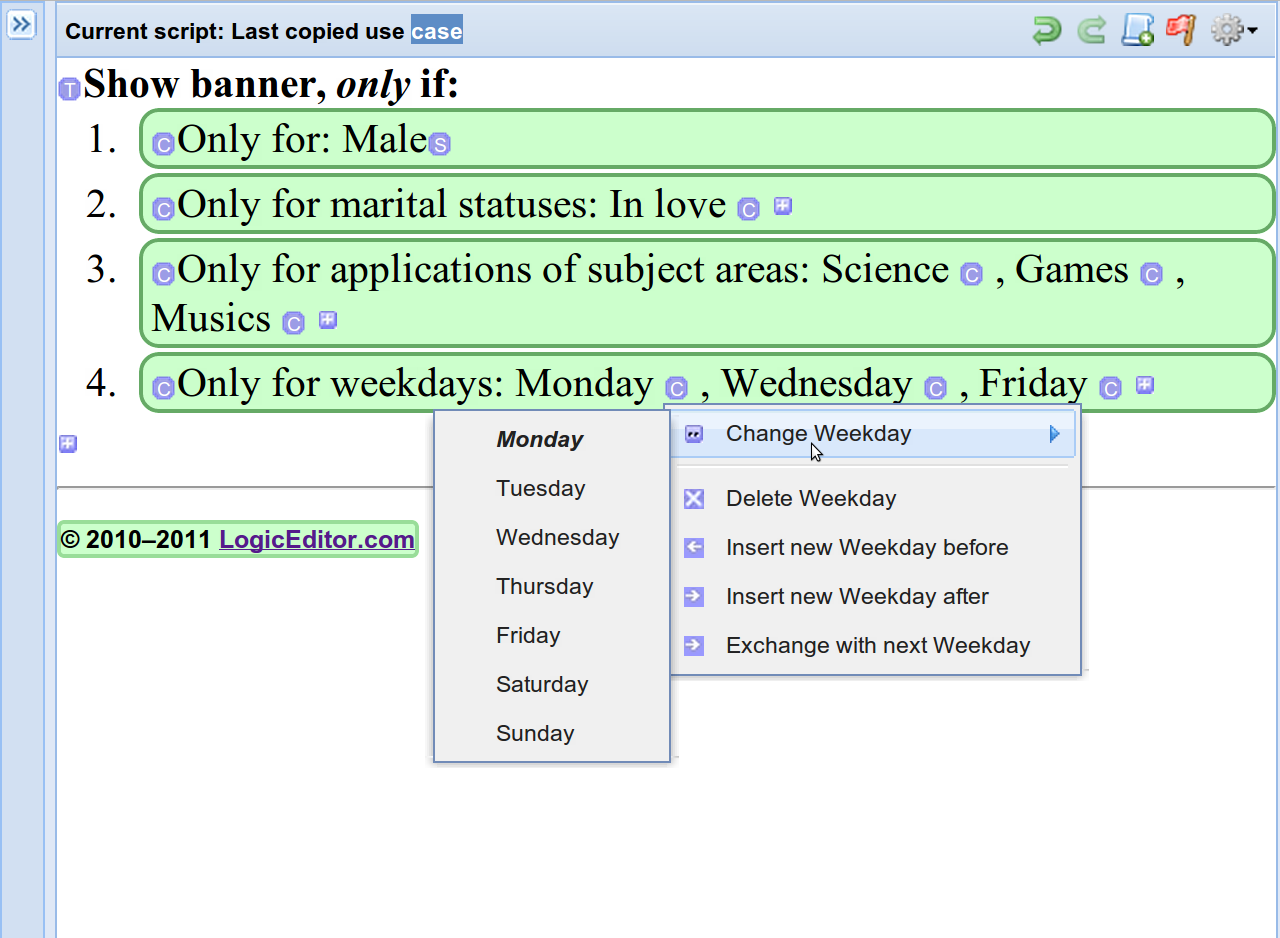
\includegraphics{logiceditor.png}}
\end{center}

\end{frame}

%% -------------------------------------------------------------------------- %%

\begin{frame}

\frametitle{The Logic Editor DSL family: output targets}

\begin{itemize}
\item From high-level DSL:
  \begin{itemize}
  \item low-level DSL;
  \item schema docs (to be implemented).
  \end{itemize}
\item From low-level DSL:
  \begin{itemize}
  \item schema-specific visual Editor UI;
  \item data validators;
  \item data-to-code generator;
  \item data upgrade code stubs to handle schema changes.
  \end{itemize}
\end{itemize}

\end{frame}

%% -------------------------------------------------------------------------- %%

\section{Why game-changing?}

%% -------------------------------------------------------------------------- %%

\begin{frame}

\frametitle{Why game-changing?}

\begin{itemize}
\item Before:
  \begin{itemize}
  \item DSL is something exotic, hard to maintain.
  \item Not much declarative code in codebase except a few special places.
  \item All declarative code in code-base totally non-reusable ad-hoc lumps of spaghetti.
  \item Code readability suffers, bugs thrive.
  \end{itemize}
\pause
\item Now:
  \begin{itemize}
  \item DSLs are much easier to write and reuse.
  \item At least 2/3 of the new code is written in DSL of one kind or another.
        (But we heavily combine declarative DSL code with Lua functions embedded in it.)
  \item Code much more readable, less bugs in generated code.
  \end{itemize}
\item In future:
  \begin{itemize}
  \item A DSL to define DSLs!
  \end{itemize}
\end{itemize}

\end{frame}

%% -------------------------------------------------------------------------- %%

\section{Questions?}

%% -------------------------------------------------------------------------- %%

\begin{frame}

\frametitle{Questions?}

Alexander Gladysh,
ag@logiceditor.com

\end{frame}

%% -------------------------------------------------------------------------- %%

\end{document}

%% -------------------------------------------------------------------------- %%
